%Nodes will double $CW(k)$ after collisions and reset it ($CW(k)=CW_{min}$) upon each transmission success, augmenting the collision probability. 
Because CSMA/ECA is totally distributed, the number of nodes ($N$) is unknown to all contenders. In the following we introduce a mechanism able to reach collision-free operation without knowledge of $N$, even for a large number of contenders.
%However the backoff stage of each station provides a hint of the level of contention.

%Therefore, $CW(k)$ is used to relate collisions to the number of users in the system.

%$N$ is unknown to all contenders, so $CW(k)$ is the only indicator for each node of the current state of the system.

To make it possible to achieve a collision-free state when the system is overcrowded, we instruct nodes not to reset $CW(k)$ after successful transmissions, and pick a deterministic backoff $B_{\mbox{\scriptsize{d}}}=CW(k)/2$. This is called \emph{hysteresis} from here on. 

%and modify the collision-free constraint to~$N_{\max}^{\mbox{\scriptsize{cf}}}=CW(k)/2$



%Hysteresis forces nodes to \emph{stick} to the value of the current backoff stage, $k$; resulting in a deterministic backoff greater than the minimum contention window.

%This measure leads to a collision-free state while $N\leq B_{\mbox{\scriptsize{d}}}$.

Hysteresis produces deterministic backoffs that are larger than $CW_{\min}/2$, thus making it possible to allocate more contenders in a collision-free fashion. Contenders may be in different deterministic backoff stages, which provokes some nodes to access the channel more often than others. This fairness issue, that can be observed in Figure~\ref{fig:fairShare}, is averted with \emph{fair-share}. The concept of fair-share, was first introduced by Fang et al. in~\cite{L_MAC2}.
%Having a greater collision-free constraint means that more nodes are able to achieve a collision-free state. 


Fair-share consist in allowing each contender to send $2^{k}$ packets at every transmission, making sure that contenders with longer backoff are compensated proportionally.

Figure~\ref{fig:fairShare}, depicts how CSMA/ECA with hysteresis and fair-share achieves greater throughput than CSMA/ECA with hysteresis only, maintaining a collision-free state while being fair (Jain's Fairness Index~\cite{JFI}~(JFI) equal to $1$), for any number of contenders.

\begin{figure}[htbp]
  \centering
  \includegraphics[width=0.7\linewidth, angle = -90]{figures/errorPlots/ECA-w-enhancements-NEW.eps}
  \caption{Throughput and Jain's Fairness Index when implementing hysteresis and fair-share in CSMA/ECA
  \label{fig:fairShare}}
\end{figure}

This work evaluates the performance of CSMA/ECA when implementing the concept in a customized C++ simulator.

\section{Evaluation}
%Other performance evaluations, like a semi-analytical framework modelling the enhanced collision avoidance mechanism and comparing it with other access schemes (like Basic Access and RTS/CTS), are provided in~\cite{E2CA_performance}. Nevertheless, to the best of our knowledge this is the first evaluation of resilience and fair-share in CSMA/ECA.

Implementation is performed on a customized version of the COST~\cite{COST}~simulator. The system was set to be under saturation (nodes always have packets to transmit) during a period of ten seconds at a maximum throughput of $11$Mbps. The number of contenders ranges from $2$ to $50$ and a hundred simulations are performed for each number of contenders. Further MAC-related parameters as well as the code for the whole CSMA/ECA implementation can be found in~\cite{sim:parameters}.

Figure~\ref{fig:throughput} and Figure~\ref{fig:fairShare} are results derived from the evaluation platform with $95\%$ confidence intervals. Note that the confidence intervals are so small that can hardly be appreciated in the figure.